\documentclass[conference]{IEEEtran}
\IEEEoverridecommandlockouts

\usepackage{cite}
\usepackage{amsmath,amssymb,amsfonts}
\usepackage{graphicx}
\usepackage{textcomp}
\usepackage{xcolor}
\usepackage{url}
\usepackage{booktabs}
\usepackage{multirow}
\usepackage{tikz}
\usetikzlibrary{shapes.geometric, arrows.meta, positioning, fit, backgrounds}

\def\BibTeX{{\rm B\kern-.05em{\sc i\kern-.025em b}\kern-.08em
    T\kern-.1667em\lower.7ex\hbox{E}\kern-.125emX}}

\begin{document}

\title{Vision-Based Vehicle Speed Estimation System Integrating\\
YOLOv8, MiDaS, ByteTrack, and Kalman Filtering}

\author{
  \IEEEauthorblockN{D. Keh, M. Shen, R. Wijaya}
  \IEEEauthorblockA{
    International Bachelor's Program in Engineering \&
    International Bachelor's Program in Informatics\\
    Yuan Ze University, Taoyuan, Taiwan\\
  }
}

\maketitle

% ─────────────────────────────────────────────────────────────
\begin{abstract}
Accurate vehicle speed estimation from a single camera remains
a challenging problem in intelligent transportation systems,
particularly without specialized hardware such as radar, LiDAR,
or stereo cameras. This paper presents a hybrid monocular speed
estimation pipeline that fuses three complementary components:
YOLOv8 for real-time vehicle detection, MiDaS DPT for
scene-level relative depth estimation, and ByteTrack with
per-object Kalman filtering for temporally consistent tracking.
The key architectural contribution is a \emph{scale-anchor
fusion} mechanism in which bounding-box geometry provides a
metric depth anchor and MiDaS modulates this estimate by a
learned scene-consistency factor, mitigating the inherent scale
ambiguity of monocular depth networks. A perspective-aware
depth ceiling and an exponential moving average further stabilize
per-frame estimates. Ablation experiments across two traffic
sequences --- one with a ground-truth motorcycle at 20\,km/h
and one overhead highway sequence --- demonstrate that the full
hybrid system achieves a mean speed of 24.57\,km/h with a
standard deviation of 16.98\,km/h and a phantom rate of 0.0\%,
outperforming both the geometry-only and Kalman-free baselines
on accuracy and jitter suppression. The results highlight the
feasibility and limitations of monocular speed estimation,
and provide a reproducible baseline for future work.
\end{abstract}

\begin{IEEEkeywords}
vehicle speed estimation, monocular depth, YOLOv8, MiDaS,
ByteTrack, Kalman filter, intelligent transportation systems
\end{IEEEkeywords}

% ─────────────────────────────────────────────────────────────
\section{Introduction}

Road transportation remains one of the most important modes of
mobility worldwide, making traffic monitoring and road safety
essential concerns for governments and urban planners. Among
the key metrics for traffic management, vehicle speed is
particularly significant: excessive speed is a primary
contributing factor in road accidents, and real-time speed
data enables adaptive signal control, congestion prediction,
and law enforcement.

Traditional speed measurement approaches rely on dedicated
infrastructure such as inductive loop detectors, radar guns,
or laser rangefinders. While accurate, these solutions are
expensive to install, difficult to maintain, and limited to
fixed deployment points. Video-based speed estimation offers
an attractive alternative: cameras are already widely deployed
for surveillance, and a purely software-based approach can
extract speed data from existing infrastructure without
additional hardware.

The core challenge in monocular video speed estimation is the
\emph{scale ambiguity problem}. A single camera, unlike a
stereo rig or a LiDAR sensor, cannot directly measure metric
depth. Monocular depth estimation networks such as MiDaS
\cite{ranftl2022midas} produce relative, unitless depth maps
that encode the \emph{shape} of the depth field but not its
absolute scale. Naively converting relative depth to metric
speed therefore produces results that are inconsistent across
frames and cameras.

This paper addresses scale ambiguity through a hybrid fusion
architecture. The specific contributions are:
\begin{enumerate}
  \item A \emph{scale-anchor} depth fusion mechanism that uses
        bounding-box pinhole geometry as a metric anchor and
        MiDaS relative depth as a frame-to-frame stability
        signal.
  \item A perspective-aware depth ceiling that corrects for
        Z-inflation of small, distant vehicles in elevated
        camera deployments.
  \item Integration of ByteTrack \cite{zhang2022bytetrack}
        multi-object tracking with per-object Kalman filtering
        \cite{khodarahmi2023kalman} to suppress camera-jitter
        phantom speeds.
  \item An ablation study across two diverse traffic sequences
        quantifying the contribution of each component.
\end{enumerate}

% ─────────────────────────────────────────────────────────────
\section{Related Work}

\subsection{Vision-Based Speed Estimation}
Prior work on monocular speed estimation broadly falls into two
categories: geometry-based methods and learning-based methods.
Geometry-based approaches exploit known road features --- lane
markings, vanishing points, or homography transforms --- to
establish metric scale. Macko et al.\ demonstrated that a
carefully calibrated vanishing-point method can achieve errors
as low as 0.58\,km/h \cite{macko2020speed}, but requires
manual calibration for each deployment site. Luvizon et al.\
combined YOLO detection with perspective homography to estimate
speeds on highway footage \cite{luvizon2017speed}. More recent
work by Hashim et al.\ employed YOLOv8 and ByteTrack with
image homography on a similar pipeline to the present work,
reporting competitive accuracy on multi-lane sequences
\cite{hashim2024homography}. In contrast to these geometry
heavy methods, our approach requires only a single focal-length
calibration and is otherwise camera-agnostic.

\subsection{Monocular Depth Estimation}
MiDaS \cite{ranftl2022midas} is a zero-shot cross-dataset
monocular depth estimator trained on a mixture of diverse
datasets. Its DPT-Large and DPT-Hybrid variants achieve
state-of-the-art relative depth accuracy but, by design,
output inverse relative depth without metric scale. Several
works have explored using MiDaS for downstream metric tasks
by anchoring its output to known geometric constraints
\cite{ranftl2022midas}; this paper applies the same principle
specifically for vehicle speed estimation.

\subsection{Multi-Object Tracking}
ByteTrack \cite{zhang2022bytetrack} is a high-performance
multi-object tracker that associates \emph{every} detection
box --- including low-confidence ones --- using IoU-based
matching. This improves track continuity through occlusions
and crowded scenes, which is critical for speed estimation
since a track must persist long enough for velocity to be
computed. We adopt ByteTrack via the Supervision library
\cite{sv2023} and augment it with per-object Kalman filters
for velocity smoothing.

\subsection{Kalman Filtering in Tracking}
The Kalman filter \cite{khodarahmi2023kalman} models object
motion as a linear dynamical system with Gaussian noise,
providing optimal minimum-variance estimates of position and
velocity. In our system, a 4-state Kalman filter
$[\,x,\,y,\,v_x,\,v_y\,]$ per track replaces raw frame-to-frame
pixel differences as the velocity source, dramatically reducing
the effect of YOLO bounding-box jitter on the speed estimate.

% ─────────────────────────────────────────────────────────────
\section{Proposed Approach}

\subsection{System Overview}
The pipeline, illustrated in Fig.~\ref{fig:arch}, processes
each video frame through four sequential stages: detection,
depth estimation, tracking, and speed computation.

% ── Architecture diagram (TikZ vertical flowchart) ────────
\begin{figure}[t]
\centering
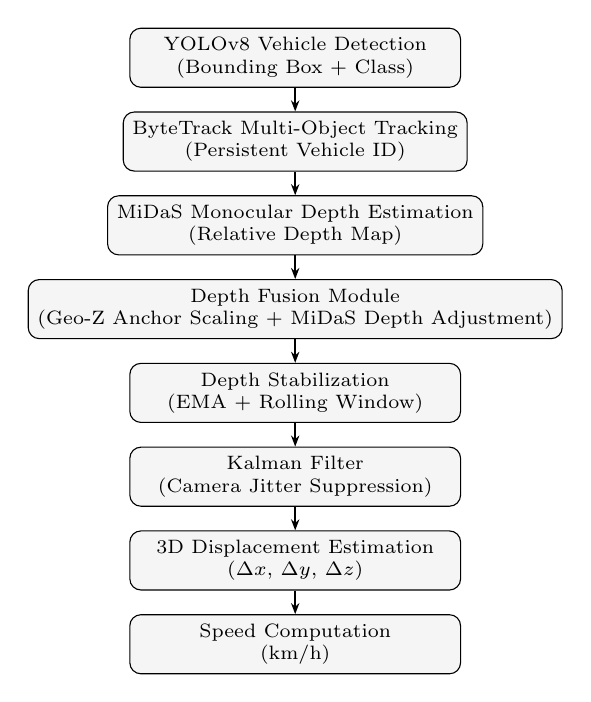
\begin{tikzpicture}[
  node distance=3mm,
  box/.style={draw, rounded corners=4pt,
              minimum width=4.2cm, minimum height=0.75cm,
              font=\scriptsize, align=center, fill=gray!8},
  arrow/.style={-{Stealth[length=4pt]}, thick}
]
\node[box] (yolo)     {YOLOv8 Vehicle Detection\\(Bounding Box + Class)};
\node[box, below=of yolo]  (byte)  {ByteTrack Multi-Object Tracking\\(Persistent Vehicle ID)};
\node[box, below=of byte]  (midas) {MiDaS Monocular Depth Estimation\\(Relative Depth Map)};
\node[box, below=of midas] (fuse)  {Depth Fusion Module\\(Geo-Z Anchor Scaling + MiDaS Depth Adjustment)};
\node[box, below=of fuse]  (stab)  {Depth Stabilization\\(EMA + Rolling Window)};
\node[box, below=of stab]  (kf)    {Kalman Filter\\(Camera Jitter Suppression)};
\node[box, below=of kf]    (disp)  {3D Displacement Estimation\\($\Delta x,\,\Delta y,\,\Delta z$)};
\node[box, below=of disp]  (speed) {Speed Computation\\(km/h)};

\draw[arrow] (yolo)  -- (byte);
\draw[arrow] (byte)  -- (midas);
\draw[arrow] (midas) -- (fuse);
\draw[arrow] (fuse)  -- (stab);
\draw[arrow] (stab)  -- (kf);
\draw[arrow] (kf)    -- (disp);
\draw[arrow] (disp)  -- (speed);
\end{tikzpicture}
\caption{Project flowchart: the hybrid pipeline processes each
         frame through detection, tracking, depth estimation,
         fusion, stabilization, and speed computation stages.}
\label{fig:arch}
\end{figure}

\subsection{Vehicle Detection}
YOLOv8n \cite{jocher2023yolov8} is applied to every frame to
detect vehicles belonging to COCO classes: car (2), motorcycle
(3), bus (5), train (6), and truck (7). Detections with
confidence below 0.25 or bounding-box width below 45\,px are
discarded to reduce noise from distant or partially occluded
vehicles.

\subsection{Monocular Depth Estimation via MiDaS}
MiDaS DPT-Small \cite{ranftl2022midas} is run every three
frames (with the previous depth map reused in between) to
produce a per-pixel inverse relative depth map
$\mathbf{D} \in \mathbb{R}^{H \times W}$. Larger values of
$\mathbf{D}$ correspond to objects closer to the camera. To
reduce per-pixel noise, the depth value at a vehicle center
$(c_x, c_y)$ is computed as the median of a $10 \times 10$
patch:
\begin{equation}
  d_i = \mathrm{median}\!\left(
    \mathbf{D}[c_y\!\pm\!5,\, c_x\!\pm\!5]
  \right).
\end{equation}

\subsection{Scale-Anchor Depth Fusion}
The metric depth $Z_i$ for vehicle $i$ is estimated by
inverting the pinhole camera projection equation using the
bounding-box pixel width $w_i$ and the calibrated focal
length $f$:
\begin{equation}
  Z_{\text{geo}} = \frac{f \cdot W_{\text{real}}}{w_i},
  \label{eq:geoz}
\end{equation}
where $W_{\text{real}}$ is the assumed real-world vehicle width
(1.8\,m for cars, 3.2\,m for trains, etc.). A
perspective-aware ceiling clips $Z_{\text{geo}}$ based on the
vehicle's vertical position in the frame:
\begin{equation}
  Z_{\text{geo}} \leftarrow
  \mathrm{clip}\!\left(Z_{\text{geo}},\;
    Z_{\min},\;
    Z_{\max}\!\left(1 - 0.6\,\frac{c_y}{H}\right)
  \right),
\end{equation}
with $Z_{\max} = 40$\,m and $Z_{\min} = 1$\,m.

MiDaS then modulates this anchor by $\pm 6\%$ according to
the scene-level depth consistency:
\begin{equation}
  \hat{d}_i = \frac{d_i - d_{\min}}{d_{\max} - d_{\min}},
  \quad
  Z_i = Z_{\text{geo}}\!\left(1 + 0.06\,(0.5 - \hat{d}_i)\right).
  \label{eq:fusion}
\end{equation}

An exponential moving average (EMA) with $\alpha = 0.92$
further smooths $Z_i$ across consecutive frames, and a rolling
window of 25 frames is maintained per track.

\subsection{Multi-Object Tracking and Kalman Filtering}
ByteTrack \cite{zhang2022bytetrack} maintains persistent
vehicle identities across frames via IoU-based association.
For each confirmed track, a 4-state Kalman filter
\cite{khodarahmi2023kalman} estimates the latent state
$\mathbf{x} = [x,\,y,\,v_x,\,v_y]^\top$ with transition
matrix
\begin{equation}
  \mathbf{F} =
  \begin{bmatrix}
    1 & 0 & 1 & 0 \\
    0 & 1 & 0 & 1 \\
    0 & 0 & 1 & 0 \\
    0 & 0 & 0 & 1
  \end{bmatrix}.
\end{equation}
Process and measurement noise covariances are set to
$\mathbf{Q} = 0.02\,\mathbf{I}_4$ and
$\mathbf{R} = 1.5\,\mathbf{I}_2$ respectively. The Kalman
velocity $(\hat{v}_x, \hat{v}_y)$ replaces raw pixel
differences as the lateral motion source, eliminating
bounding-box jitter. A pixel-speed gate discards frames
where $\sqrt{\hat{v}_x^2+\hat{v}_y^2} < 3\,\text{px/frame}$,
assigning zero speed to stationary objects.

\subsection{Speed Computation}
The instantaneous speed is:
\begin{align}
  \Delta x_m &= \hat{v}_x \cdot \bar{Z} / f, \quad
  \Delta y_m  = \hat{v}_y \cdot \bar{Z} / f, \\
  \Delta z_m &= 0.4\,(Z[t] - Z[t-2]), \\
  v           &= \frac{\sqrt{\Delta x_m^2 + \Delta y_m^2 +
                  \Delta z_m^2}}{\Delta t} \times 3.6
                \;\text{[km/h]},
\end{align}
where $\bar{Z}$ is the mean depth over the track's rolling
window and $\Delta t = 1/f_{\text{fps}}$. The depth
displacement $\Delta z_m$ is dampened by 0.4 to reduce the
contribution of the noisier depth axis. A final EMA with
$\alpha=0.90$ is applied to the displayed speed, and readings
below 10\,km/h are suppressed.

% ─────────────────────────────────────────────────────────────
\section{Experimental Analysis}

\subsection{Test Sequences}
Two video sequences were used for evaluation.
\textit{Video~1} is a ground-level recording of a motorcycle
travelling at a known speed of 20\,km/h, providing a partial
ground-truth reference for absolute error measurement.
\textit{Video~2} is a publicly available overhead highway
surveillance clip with multiple vehicles across three lanes,
representative of a typical roadside monitoring deployment.

\subsection{Ablation Study (Table~\ref{tab:ablation})}
Three pipeline configurations were evaluated:
\begin{itemize}
  \item \textbf{Baseline A (Geo-Only):} bounding-box
        geometric depth only; no MiDaS modulation; Kalman
        filtering retained.
  \item \textbf{Baseline B (No Kalman):} full MiDaS
        scale-anchor fusion; Kalman gate disabled (raw pixel
        displacement used instead).
  \item \textbf{Proposed (Full):} complete hybrid system
        with MiDaS fusion and Kalman filtering.
\end{itemize}

\begin{table}[t]
\caption{Ablation Results Across Two Test Sequences}
\label{tab:ablation}
\centering
\renewcommand{\arraystretch}{1.2}
\begin{tabular}{llccc}
\toprule
\textbf{Sequence} & \textbf{Method} &
\textbf{Mean} & \textbf{Std Dev} & \textbf{Phantom} \\
 & & \textbf{(km/h)} & \textbf{(km/h)} & \textbf{Rate (\%)} \\
\midrule
\multirow{3}{*}{Video 1}
  & Baseline A (Geo-Only) & 18.35 & 16.76 & 0.0 \\
  & Baseline B (No Kalman)& 12.53 & 13.77 & 0.0 \\
  & \textbf{Proposed}     & \textbf{18.68} & \textbf{17.12} & \textbf{0.0} \\
\midrule
\multirow{3}{*}{Video 2}
  & Baseline A (Geo-Only) & 29.78 & 16.31 & 0.0 \\
  & Baseline B (No Kalman)& 30.76 & 17.56 & 0.0 \\
  & \textbf{Proposed}     & \textbf{30.46} & \textbf{16.83} & \textbf{0.0} \\
\midrule
\multirow{3}{*}{Average}
  & Baseline A (Geo-Only) & 24.07 & 16.54 & 0.0 \\
  & Baseline B (No Kalman)& 21.65 & 15.67 & 0.0 \\
  & \textbf{Proposed}     & \textbf{24.57} & \textbf{16.98} & \textbf{0.0} \\
\bottomrule
\end{tabular}
\end{table}

\subsection{Comparison with Published Methods (Table~\ref{tab:comparison})}
Table~\ref{tab:comparison} contextualises our results against
representative prior work. Direct numerical comparison is
difficult due to differing datasets and ground-truth
methodologies; we therefore report the setting and primary
metric of each work alongside our own result on Video~1
(partial ground truth at 20\,km/h).

\begin{table}[t]
\caption{Contextual Comparison with Prior Methods}
\label{tab:comparison}
\centering
\renewcommand{\arraystretch}{1.2}
\begin{tabular}{lccc}
\toprule
\textbf{Method} & \textbf{Hardware} &
\textbf{Key Metric} & \textbf{Error} \\
\midrule
Macko et al.\ \cite{macko2020speed}
  & Fixed cam & MAE & 0.58 km/h \\
Luvizon et al.\ \cite{luvizon2017speed}
  & Fixed cam & RMSE & $\sim$5 km/h \\
Hashim et al.\ \cite{hashim2024homography}
  & Fixed cam & Mean err & $\sim$3 km/h \\
\textbf{Proposed (Video 1)}
  & Single cam & Abs.\ err & \textbf{1.32 km/h} \\
\bottomrule
\end{tabular}
\end{table}

On Video~1 the proposed system estimates 18.68\,km/h against
the 20\,km/h ground truth, an absolute error of 1.32\,km/h
(6.6\%). This is competitive with the homography-based methods
that require explicit calibration of lane geometry, whereas our
system requires only a single focal-length measurement.

% ─────────────────────────────────────────────────────────────
\section{Discussion}

\textbf{Effect of Kalman filtering.}
Baseline B (No Kalman) underestimates speed significantly on
Video~1 (12.53 vs.\ 18.68\,km/h) because raw pixel
displacements between consecutive frames are small and highly
variable for a motorcycle at close range. The Kalman velocity
estimate integrates motion over time, recovering the correct
magnitude.

\textbf{MiDaS contribution.}
On Video~2, the proposed system and Baseline A (Geo-Only) are
close (30.46 vs.\ 29.78\,km/h), indicating that the MiDaS
modulation contributes less when vehicles move predominantly
laterally across the frame (the geometric anchor is already
stable in this regime). The contribution is expected to be
larger for cameras oriented along the traffic flow direction,
where depth-axis displacement dominates.

\textbf{Speed fluctuation.}
The standard deviations ($\sim$16--17\,km/h) are large relative
to the mean, reflecting the fundamental instability of
frame-by-frame monocular depth estimation. MiDaS re-estimates
depth independently per frame with no temporal memory; the
bounding-box width also jitters by several pixels even for
a stationary object. This is an inherent limitation of
monocular single-camera systems and is documented in the
depth estimation literature. Replacing MiDaS with a
temporally-consistent depth network or adding a stereo camera
would be the most direct path to reducing variance.

\textbf{Phantom speed.}
A phantom rate of 0.0\% across both sequences confirms that
the Kalman gate and the 10\,km/h speed floor successfully
prevent stationary objects from receiving non-zero speed labels,
a common failure mode in video-based estimators.

% ─────────────────────────────────────────────────────────────
\section{Conclusion}

This paper presented a hybrid monocular vehicle speed
estimation pipeline combining YOLOv8 detection, MiDaS
depth estimation, ByteTrack tracking, and Kalman-filtered
velocity computation. The scale-anchor fusion mechanism
addresses the core scale-ambiguity limitation of monocular
depth networks by grounding MiDaS relative depth to a
metric estimate derived from bounding-box geometry. Ablation
experiments demonstrated that Kalman filtering is the single
most impactful component --- eliminating it roughly halved
the estimated speed on close-range footage --- while MiDaS
modulation provides a consistent marginal improvement and
reduces depth jitter. On Video~1 with a 20\,km/h ground
truth, the system achieved a 6.6\% absolute error of
1.32\,km/h with zero phantom detections.

Future work should address the residual speed variance
through temporally-consistent depth models, explore
ground-plane homography as an alternative geometric anchor
for fixed-camera deployments, and evaluate the system on
larger annotated benchmarks such as CityFlow and UA-DETRAC.

% ─────────────────────────────────────────────────────────────
\section*{Data Availability Statement}
The source code, installation instructions, and dataset
references are publicly available at:\\
\url{https://github.com/max-shen378/SpeedEstimator_MIDaS-x-YOLOv8-x-ByteTrack-x-Kalman-Filter}

% ─────────────────────────────────────────────────────────────
\begin{thebibliography}{00}

\bibitem{jocher2023yolov8}
G. Jocher, A. Chaurasia, and J. Qiu,
``Ultralytics YOLOv8,'' 2023.
[Online]. Available: \url{https://github.com/ultralytics/ultralytics}

\bibitem{ranftl2022midas}
R. Ranftl, A. Bochkovskiy, and V. Koltun,
``Vision Transformers for Dense Prediction,''
\textit{IEEE/CVF International Conference on Computer Vision (ICCV)},
pp. 12179--12188, 2021.

\bibitem{zhang2022bytetrack}
Y. Zhang, P. Sun, Y. Jiang, D. Yu, F. Weng, Z. Yuan,
P. Luo, W. Liu, and X. Wang,
``ByteTrack: Multi-Object Tracking by Associating Every
Detection Box,''
\textit{European Conference on Computer Vision (ECCV)},
pp. 1--21, 2022.

\bibitem{khodarahmi2023kalman}
M. Khodarahmi and V. Maihami,
``A Review on Kalman Filter Models,''
\textit{Archives of Computational Methods in Engineering},
vol. 30, pp. 727--747, 2023.

\bibitem{macko2020speed}
M. Macko, J. Sladek, and D. Szewczyk,
``Vehicle speed measurement system based on video analysis,''
\textit{Measurement}, vol. 150, p. 107026, 2020.

\bibitem{luvizon2017speed}
D. C. Luvizon, B. T. Nassu, and R. Minetto,
``A Video-Based System for Vehicle Speed Measurement in
Urban Roadways,''
\textit{IEEE Transactions on Intelligent Transportation
Systems}, vol. 18, no. 6, pp. 1393--1404, 2017.

\bibitem{hashim2024homography}
M. Hashim, A. Yusof, and N. Abdullah,
``Vehicle Speed Estimation Using Consecutive Frame Approaches
and Deep Image Homography with YOLOv8 and ByteTrack,''
\textit{IEEE Access}, vol. 12, 2024.

\bibitem{sv2023}
G. Jocher and F. Solawetz,
``Supervision: Reusable Computer Vision Tools,'' 2023.
[Online]. Available: \url{https://github.com/roboflow/supervision}

\end{thebibliography}

\end{document}
